\documentclass[]{article}
\usepackage[english]{babel}
\usepackage{graphicx}
\usepackage{amsmath}
\usepackage{hyperref}

\date{Universitat Pompeu Fabra, 2017}
%opening
\title{Using basic pattern recognition techniques to solve classification and dimensionality reduction problems.}
\author{Diego \textsc{rodriguez}}

\begin{document}

\maketitle

\begin{abstract}
In this report, basic pattern recognition (PR) techniques such as the Bayesian Theorem, Multivariate Gaussian Mixture Model and Principal Component Analysis are used to solve exercises from Seminar 1 of the Pattern Recognition class.
\end{abstract}

\section{Fundamental Concepts}

Find an example in order to explain all of these concepts:

\subsection{Feature}

Let's imagine we want to construct a handwriting digit recognizer. Somehow using advanced pattern recognition techniques we are able to indentify the number of straight horizontal lines in each sample containing a number. These straight horizontal lines are **features**.

\subsection{Supervised Learning}

An example of supervised learning is a prediction model. Imagine a dataset where you want to predict if a house is going be sold based on its price and the average income of a household of the zone where the house is, such as:

\begin{center}
\begin{tabular}{c | c | c}
	House price & Average income & Was it sold?\\
	120000      & 24000 		 & Yes\\
	135000		& 30000			 & Yes\\
	180000		& 24000			 & No\\
\end{tabular}
\end{center}

You could feed a learning algorithm to learn about the $n$ features that contribute to a house being sold and try to predict if it's going get sold.

\subsection{Classification}

Try to predict if a picture contains a cat or a tiger.

\subsection{Regression}

Try to predict stock prices or estimate the remaining battery left in a phone based on several features.

\subsection{Unsupervised Learning}

Try to classify $n$ amount of people into $m$ groups. For example, you have a dataset of height and weight of your clients and you want to create the best fit for S, M, and L kind of clothes for them. Clustering would be a good approach.

\subsection{Clustering}

Clustering is an unsupervised learning technique used to automatically classify unlabeled data into groups, also known as clusters. After that, this new data can be used to improve the algorithm.

\section{Bayesian Theorem}

Walking through the jungle, you see a large feline shadow. However, you can not identify what animal it is. You know that, in this area of the jungle, 90\% of felines are not dangerous cats whereas the other 10 \% are pumas . In addition, you know that 80\% of cats are smaller than the animal you are seeing whereas 85\% of pumas has a similar size. Would you run?\\

\textbf{Reminder}: We define Bayes Theorem as follows $p(A|B) = \frac{p(B|A)p(A)}{p(B)}$, where $A, B$ are events and $p(B) \neq 0$\\

Let $A$ denote the event of feline being dangerous. Let $B$ denote the event of watching a big feline with similar size to pumas and bigger than 80\% of cats. We know that the probability of any random given feline of being a puma is 0.1 and any random feline of being a cat is 0.9. Also, we know that 85\% of pumas can be a big feline like the one watched and that at most, 20\% of cats are like that big feline:\\

$$p(A) = 0.1$$
$$p(B) = 0.1 \cdot 0.85 + 0.9 \cdot 0.2 = 0.265$$

Then, the probability of  watching a big feline ($B$) **knowing** that the feline is a puma ($A$) is defined as:\\

$$p(B|A) = 0.85$$

Using Bayes Theorem we can calculate the probability of a feline being a puma given the event that we see a big feline: $p(A|B)$\\

$$p(A|B) = \frac{p(B|A)p(A)}{p(B)} = \frac{0.85 \cdot 0.1}{0.265} = 0.32$$

\textsc{Indeed, I would run}.

\section{Gaussian Model}

Following the last example, assume that the variable size is continuous.
\begin{itemize}
\item Draw a figure (approximated) of the distribution functions p(size | cat) and p(size | puma). To do so, assume that the size of cats and pumas follow a normal distribution where cat’s size tend to be smaller than pumas. Moreover, you know that the size of different cat species use to be more variable than in the case of pumas.

\item Over the same figure, and following the Bayesian Decision Theory, draw the 2 decision regions which classify cats and pumas with respect to their size. Draw also the region which corresponds to the decision error.
\end{itemize}

To do the figure I used Matlab. I implemented a script that assumes the values of $\mu_1$ = 40 and $\mu_2$ = 70, $\sigma_1$ = 12 and $\sigma_2$ = 7. Where the sub-indexes 1 and 2 denote the cat and puma population parameters respectively. \\

Using the script \texttt{exercise\_3.m} with $\mu_1 = 40$, $\mu_2 =  70$, $\sigma_1 = 12$ and $\sigma_2 = 7$:

\begin{figure}[ht!]
\centering
	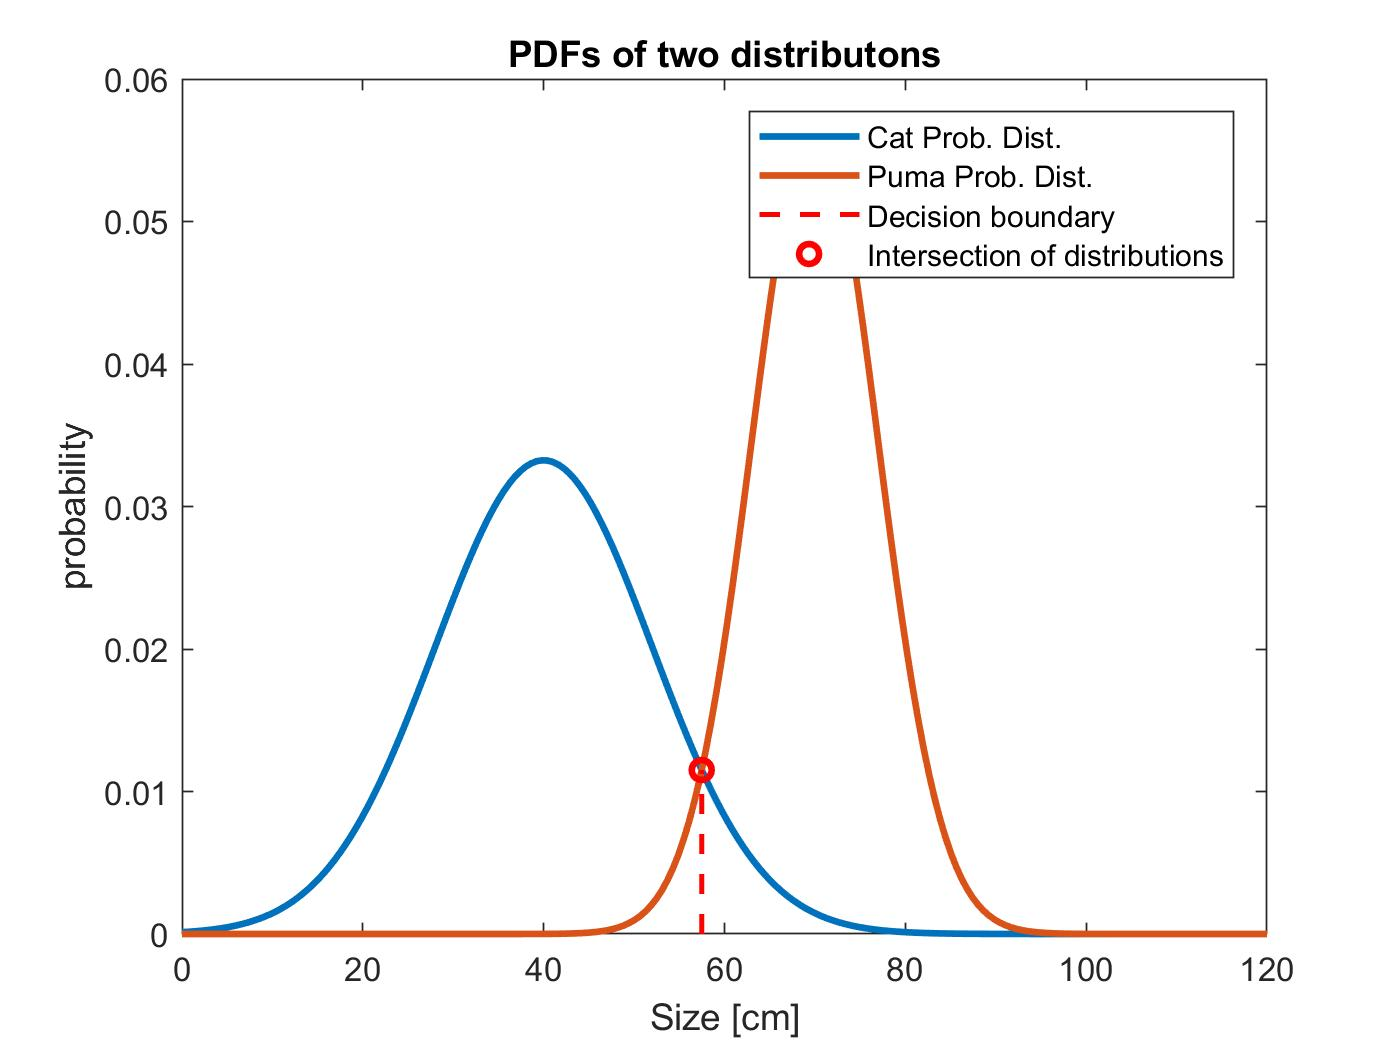
\includegraphics[width=0.5\textwidth]{../img/1d-gauss-model}
	\caption{Probability density functions of the two feline distributions}
\end{figure}

We know that the intersection point of both distribution located \textbf{in between}, corresponds to the point of maximum uncertainty because there is a 50\% chance of being one population or the other just based on the size variable. To the left of the decision boundary we predict cats, and to the right we predict puma; the more a value approaches the peaks of both distributions the higher the confidence.

\begin{figure}[ht!]
\centering
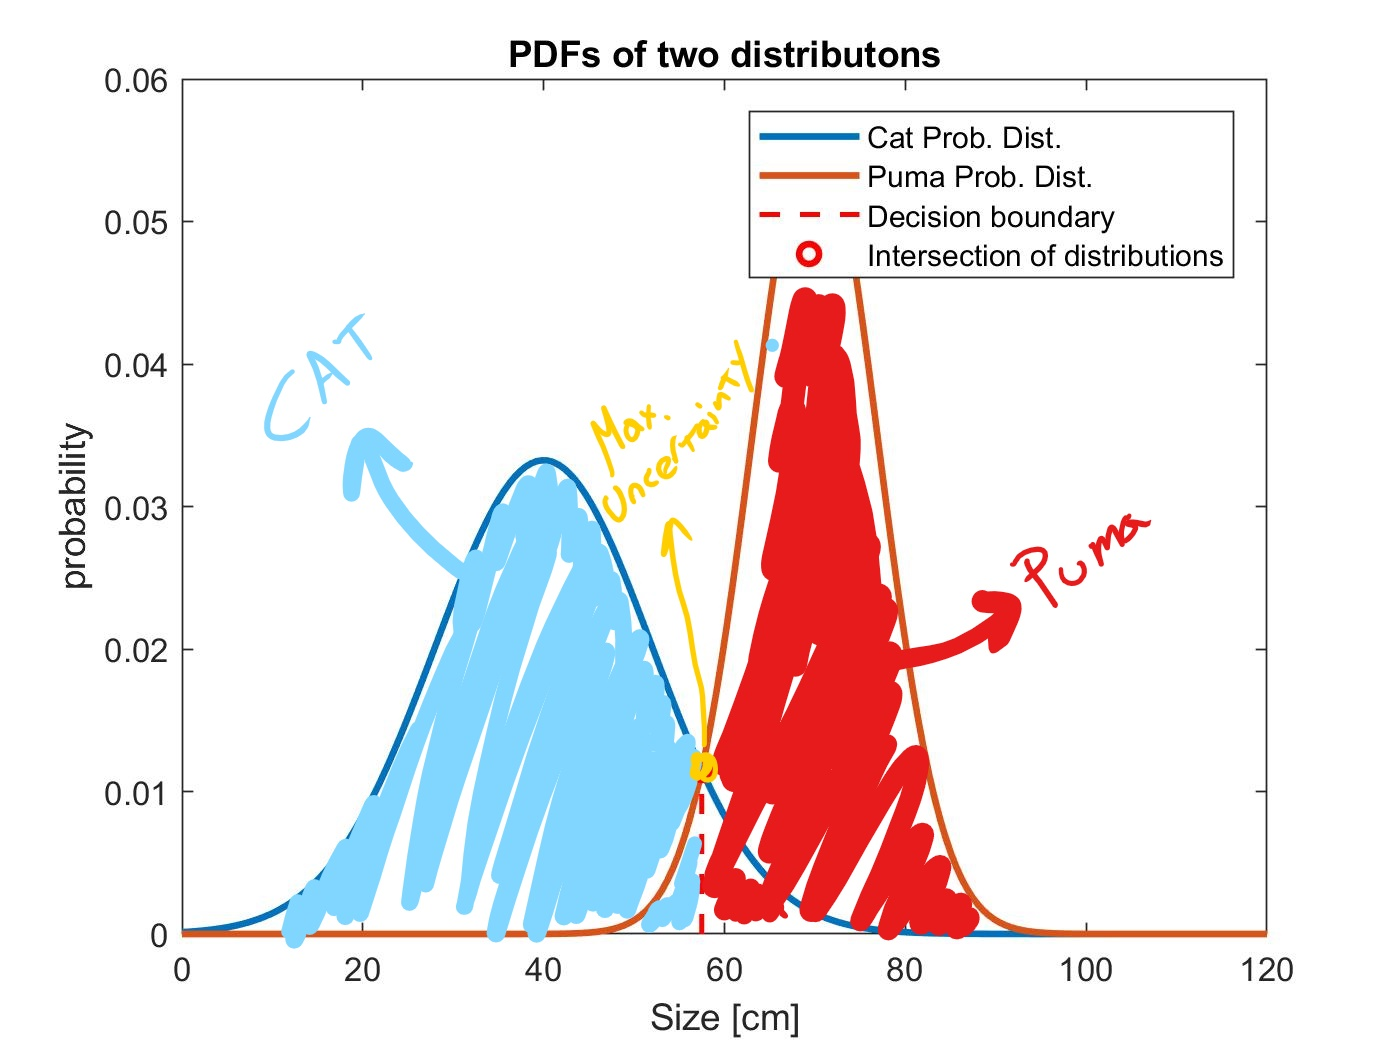
\includegraphics[width=0.5\textwidth]{../img/1d-gauss-model-ink}
\caption{Prediction Regions}
\end{figure}

\section{Same variance gauss model}
Assume that probabilities $p(size|cat)$ and $p(size|puma)$ follow two normal distributions $N(\mu_1 , \sigma )$ and $N(\mu_2, \sigma)$ respectively. Given that $p(cat) = p(puma) = 0.5$ and $\sigma_1 = \sigma_2$, find the size value x* which corresponds to the decision boundary classifying cats or pumas. Define x* as a function of $\mu_1$ and $\mu_2$.\\

Using the same variances $\sigma_1 = \sigma_2 = 12$, the size would be 55cm as shown on the figure:

\begin{figure}[ht!]
\centering
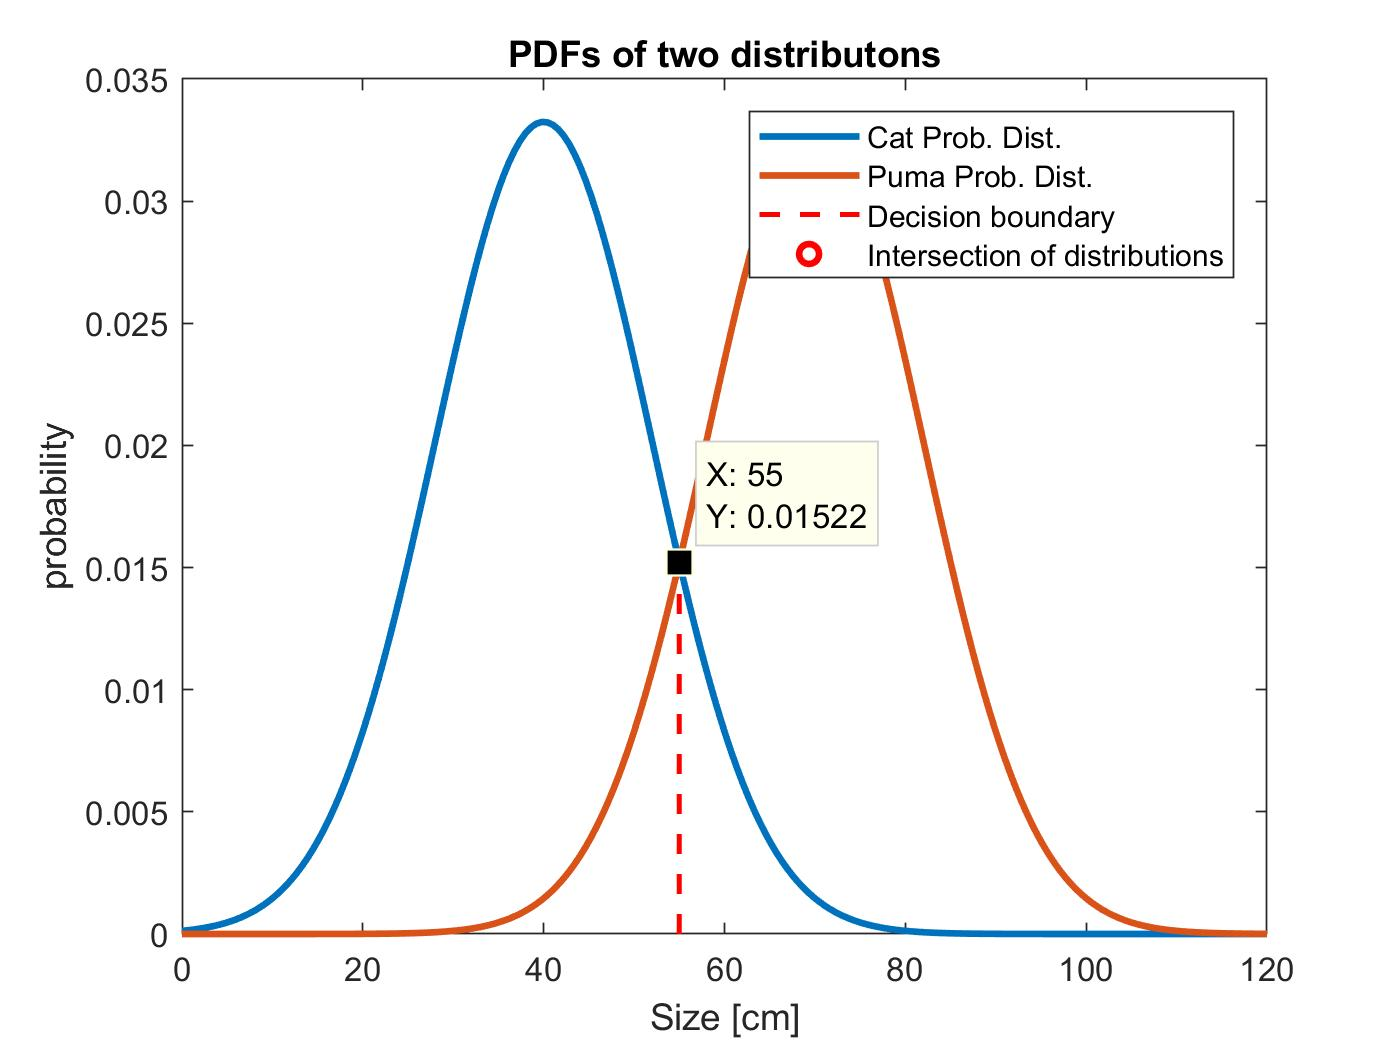
\includegraphics[width=0.5\textwidth]{../img/1d-gauss-model-same-mean}
\caption{Using same variance.}
\end{figure}

\section{Multi-Variate Gaussian Mixture Model}

Imagine that you have a hen and a goose in your home. One day, you find an egg but you do not know who have laid it. You measure the weight and the height of the egg, which are 60g and 5cm respectively. Assuming that the laying frequency of the chickens is the double than the gooses one, and the following mean and covariance matrices:

\[
\sigma_1 = 
\begin{pmatrix}
5 & \frac{1}{10} \\ 
\frac{1}{10} & \frac{1}{2}
\end{pmatrix} 
\]

\[
\sigma_2 = 
\begin{pmatrix}
8 & \frac{1}{5} \\ 
\frac{1}{5} & 1
\end{pmatrix} 
\]
\[ \mu_1 = (54, 5)\]
\[\mu_2 = (65, 6)\]

What we have to do is calculate the probability density function (pdf)
of the two distributions. One pdf for the chicken eggs and another one
for the goose eggs. However, this time we have two variables, weight and
size, so we have to use the multivariate gaussian pdf, given by the
formula:

\begin{equation}
pdf(x, \mu, \Sigma) = \operatorname{det}(2\pi\boldsymbol\Sigma)^{-\frac{1}{2}} \, e^{ -\frac{1}{2}(\mathbf{x} - \boldsymbol\mu)'\boldsymbol\Sigma^{-1}(\mathbf{x} - \boldsymbol\mu) }
\end{equation}

So we just have to compute the pdf of the sample in both pdf distributions (chicken and goose), compare
the probabilities and predict the one with a higher pdf. The probability
of predicting correctly given distribution 1, as it was explained on the
last exercise, is done by taking the pdf of distribution A and dividing
it by the sum of the pdfs of all the distributions. That is:
\begin{equation}
p = \frac{pdf_1(s)}{\sum_{i = 0}^{N}{pdf_i(s)}}
\end{equation}

Using Matlab script \texttt{exercise\_5.m} we can
easily visualize the results:

\pagebreak

\begin{figure}[h!]
\centering
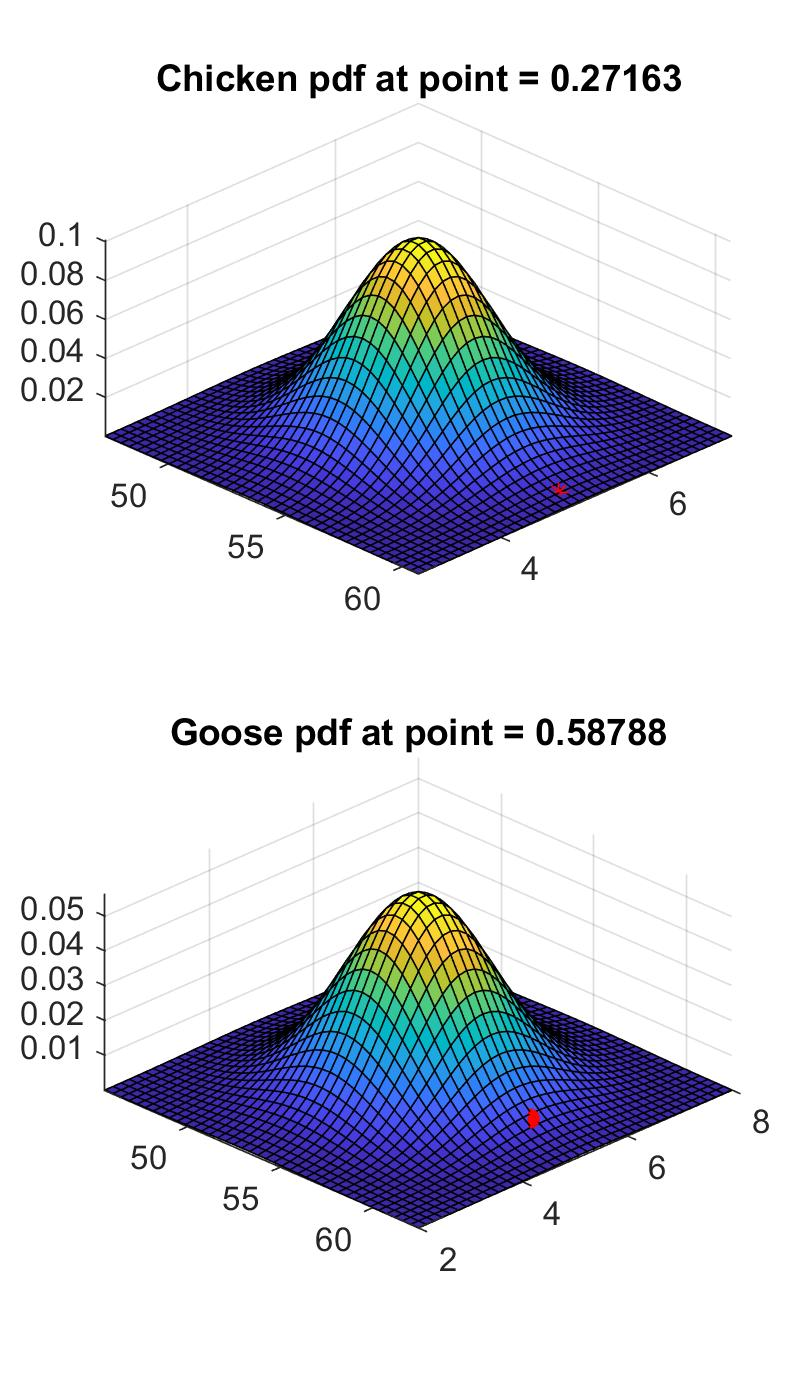
\includegraphics[width=0.5\textwidth]{../img/2d-gauss-model}
\caption{2-Variable Gaussian Model Representation, the z-axis represents the pdf. Top view of this same representation, open file: \texttt{2d-gauss-model-top.jpg} in the \texttt{img} folder.}
\end{figure}

Then, since goose pdf is higher we predict is from a goose. To calculate the probability or confidence of the egg belonging to the goose distribution we use equation (2):

$$
p_c = \frac{0.58788}{0.58788 + 0.27163} \approx 0.68 \rightarrow 68\% \text{ confidence}.
\pagebreak
$$
\section{Fisher's Database}

Download the data from the dataset that you will find in uci.edu\footnote{https://archive.ics.uci.edu/ml/datasets/Iris}. Use it to classify the following unlabeled samples:

%| Sepal length | Petal length | Sepal width | Petal width |
%|--------------|--------------|-------------|-------------|
%| 4,9          | 3,2          | 1,7         | 0,2         |
%| 5            | 3,2          | 1,6         | 0,5         |
%| 5,5          | 2,8          | 3,6         | 1,3         |
%| 7,1          | 3,1          | 6,1         | 1,7         |

\begin{center}
	\begin{tabular}{c | c | c | c}
		\textbf{Sepal length} 	& \textbf{Petal length} 	& \textbf{Sepal width} 	& \textbf{Petal width}\\
		4.9				& 3.2			& 1.7			& 0.2\\
		5				& 2.8			& 1.6 			& 0.5\\
		5.5				& 2.8			& 3.6			& 1.3\\
		7.1				& 3.1			& 6.1			& 1.7\\
	\end{tabular}
\end{center}

Using Matlab we just have to do the following procedure: understand the data, after that, subdivide it into different subsets (There are 3 classes), then calculate the parameters of the Gaussian distribution for each class (assuming all the three classes follow the normal distribution), so we calculate the mean $\mu$ and the covariance matrix $\Sigma$ for all the variables for each distribution. After that using equation (1) we can calculate the pdf for each distribution and then we can compare each of the pdf for each distribution and predict the one with the highest pdf value. To calculate the probabilities of our prediction we do the same as in the previous exercise. It's important to recall that we are estimating the values of $\mu, \Sigma$. That is why in real-world applications usually the more data we have the better our model will be. Executing the matlab script \texttt{exercise\_6.m} we get the following output:

\begin{verbatim}
Reading samples...
The sample 1 is a setosa. Confidence: 100 %
The sample 2 is a setosa. Confidence: 100 %
The sample 3 is a versicolor. Confidence: 99.9972 %
The sample 4 is a virginica. Confidence: 99.9289 %
\end{verbatim}
\pagebreak
\section{Principal Component Analysis (PCA)}
Suppose that we have a set of 2D samples: [0, 0], [1, 1], [2, 3], [3, 2] and [4, 4].
\begin{itemize}
	\item Draw the data and compute the covariance matrix.
	\item Apply PCA over these samples and find the basis where the data have the maximum variance. To do so, find the eigenvalues and eigenvectors of the data covariance matrix. Draw these basis in the same figure than the previous exercise.
	\item Project the data over the obtained basis with PCA. Discuss the relation existing between the covariance of the projected data and the eigenvalues computed in b).
	\item Project and re-project the data using only the basis of maximum variance. Draw the results over the original data.
\end{itemize}

All of this exercises were done at the same time. To do it I applied a very elemental PCA algorithm (not generalized) to this exercise and it plots the data, finds a new basis, plots a line along that new direction and reprojects the data:

The algorithm can be found in the \texttt{exercise\_7\_1.m} file and prints the following output:

\begin{verbatim}
1. Draw the data
2. Compute the covariance matrix

covarMat =

0.6250    0.5625
0.5625    0.6250

3. Apply PCA and find the basis:

eigenVector =

-0.7071    0.7071
0.7071    0.7071


eigenValue =

0.0625  	0
0    		1.1875

We take the vector with the highest eigenValue.
Highest Eigenvalue: 1.1875
Max. var. Eigenvector / new basis: [0.70711     0.70711]

dimReduction =

0    1.4142    3.5355    3.5355    5.6569


projected_X =

0    1.0000    2.5000    2.5000    4.0000
0    1.0000    2.5000    2.5000    4.0000
\end{verbatim}

It's important to notice that \texttt{dimReduction} values are the projected data points in the new basis found. Also, to compute the covariance matrix we just normalize the $X$ values in our dataset by doing $Z = \frac{X - \mu}{\text{range}}$ where $\text{range} = \left(\max{X} - \min{X}\right)$, although we can apply PCA without normalizing (the first implementation worked without this step), when using more advanced techniques such as gradient descent or stochastic gradient descent, this helps the algorithms converge faster and since the values are in a more narrower spectrum, the algorithms tend to be more computationally efficient, specially if using a high level language like Python or Matlab / Octave. To obtain the eigenvector I used Matlab's eigen-decomposition algorithm, although you can use single-value decomposition as well.

\begin{figure}[ht!]
	\centering
	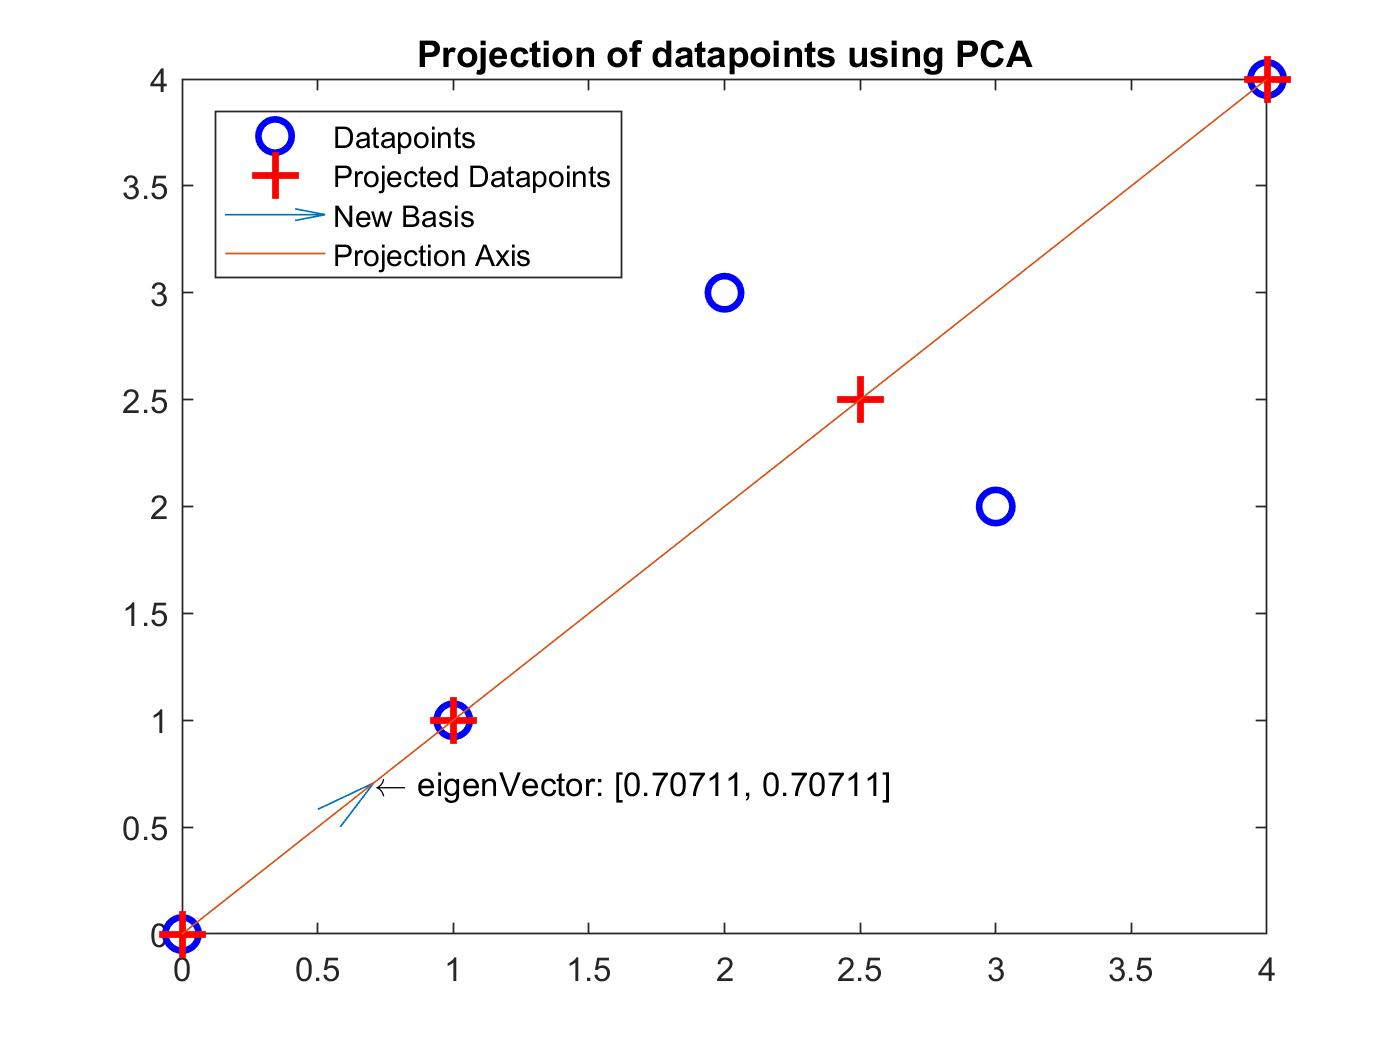
\includegraphics[width=\textwidth]{../img/pca-fig-1}
	\caption{PCA implementation with new basis projected, re-projected data-points and first principal component (first eigenvector).}
\end{figure}

\pagebreak

\section{PCA changing coordinates system}

Repeat the previous exercise with the Cartesian samples [0, 1], [0, -1], [1, 0], [-1, 0] but using cylindrical coordinates (you first have to transform the data to cylindrical coordinates\footnote{I used polar coordinates since representing 2D data-points using a 3D coordinate system is redundant and another advantage of using polar coordinates is that they allow to visualize better the exercise dynamics}). 

Using the same dynamics as the previous exercise but converting from cartesian coordinates to polar coordinates I got interesting results, data-points that were far from the original datapoints without the dimensionality reduction but that had the most variable information, the angle, so by adding the mean of the radius the exact points were recovered just by using an offset, but with 1 dimension less (The code can be found at \texttt{exercise\_8.m}), the output of the script plus the figure summarizes the quantitative results.

\pagebreak

\begin{figure}[h]
	\centering
	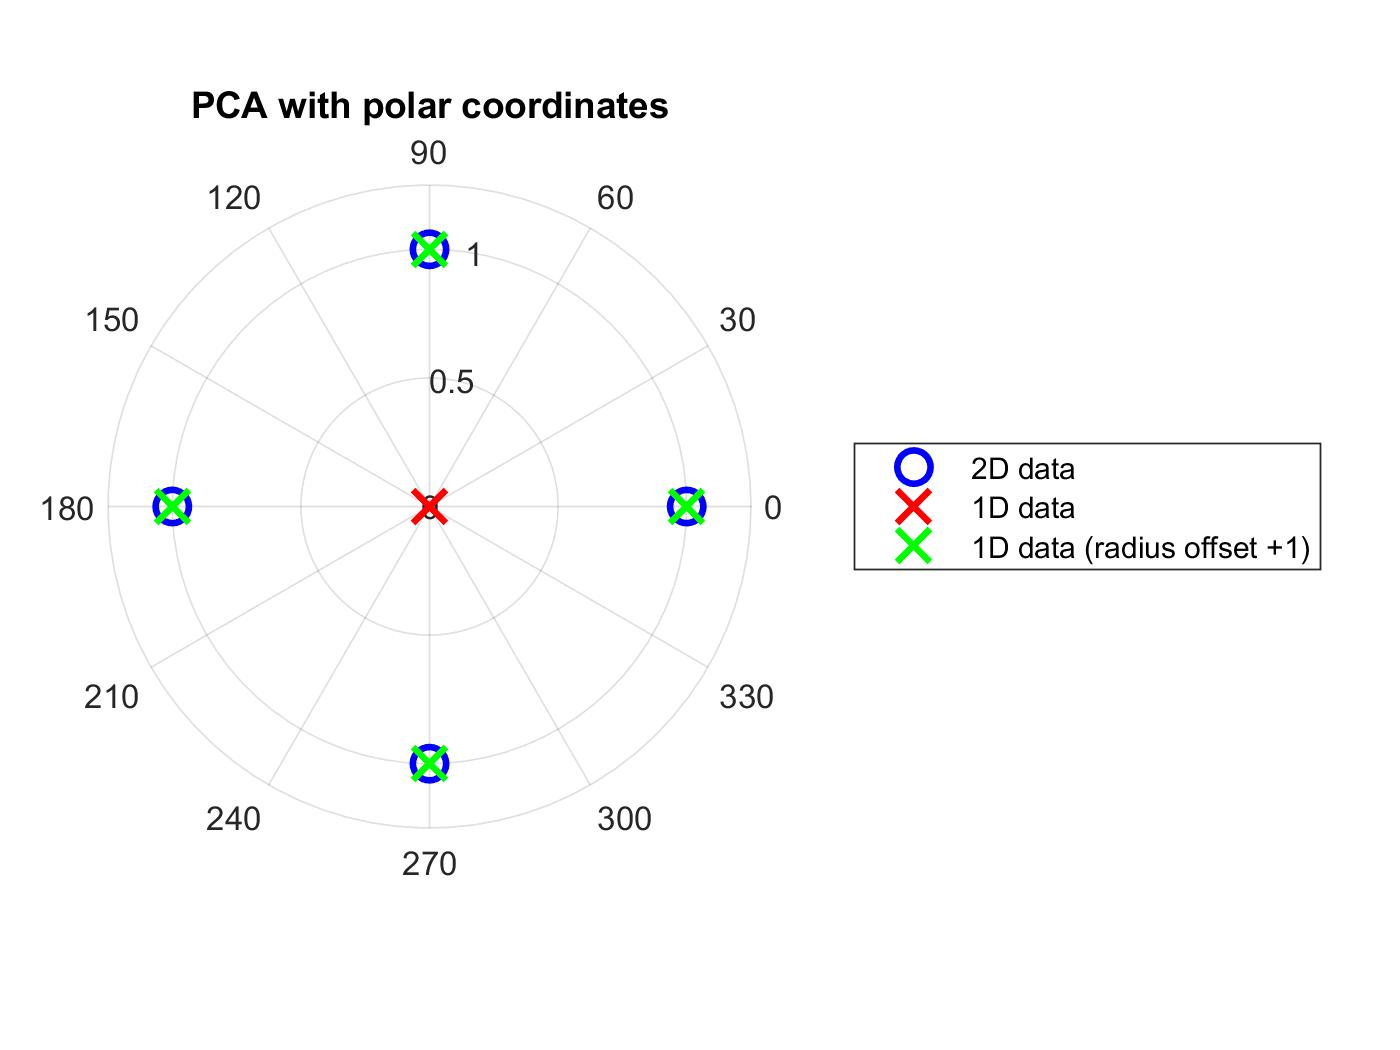
\includegraphics[width=\linewidth]{../img/pca-polar}
	\caption{Using PCA with non-linear data by changing the coordinate system}
	\label{fig:pca-polar}
\end{figure}

\textbf{Script output}:

\begin{verbatim}

dataset =

0     0     1    -1
1    -1     0     0

We go from cartesian to polar...

dataset =

1.5708   -1.5708         0    3.1416
1.0000    1.0000    1.0000    1.0000


covariance_mat =

0.5556         0
0         0


eigenVector =

0     1
1     0


eigenValue =

0         0
0    0.5556

We take the vector (in our new polar space) with the highest eigenValue.
Highest Eigenvalue: 0.55556
Max. var. Eigenvector / new basis: [1  0]

dimReduction =

1.5708   -1.5708         0    3.1416


projected_data =

1.5708   -1.5708         0    3.1416
0         0         0         0
\end{verbatim}

\pagebreak

\section{PCA + Multi Variate Gaussian Model}

Apply PCA to the data from exercise 6 and classify again the unlabeled samples using the Multivariate Gaussian Mixture Model with the two more significant “new attributes” found with the PCA.

This exercise summarizes all the seminar. You start by extracting the dataset, then you apply PCA and keep the 2 principal components, after that you use these 2 new principal components as your new dataset and apply multi-variate gaussian model to this two and using the pdf for each class you compare and predict. The accuracy shrinked (as expected since we now have less features), but it did so in less than 1\% which means the two features picked were really good.

The code can be found at \texttt{exercise\_9.m} and its output is:

\begin{verbatim}
Reading samples...
Applying PCA...
Using 2 out of 4 features...
97.7632% variability retained
The sample 1 is a setosa. Confidence: 100 %
The sample 2 is a setosa. Confidence: 100 %
The sample 3 is a versicolor. Confidence: 99.9823 %
The sample 4 is a virginica. Confidence: 99.9457 %
\end{verbatim}

\section{References and detailed work}

To see the source code and all the very detailed explanation of each of the steps, check-out the Jupyter Notebook at \url{https://goo.gl/J1e7Cd}\\

\centering

\textsc{THE END.}

\end{document}
